
In this work three different setups were used to obtain the permittivity of the materials in question and to characterize the waveplates. Each setup implements a different emitter-detector pair which in turn means that the frequency region with the maximum SNR varies depending on the setup. The frequency range in which we can reliably extract the optical parameters therefore varies depending on the setup. 

\section{THz-TDS TeraFlash setup}
The THz-TDS TeraFlash system is based on a \SI{1560}{\nano \meter} fiber laser which has its output split by a 50/50 fiber splitter into a detector and emitter branch, each branch is then subsequently coupled into one of two mechanical delay stages. These components are all housed in a sealed off box which further has two fiber interfaced outputs for the optical pulses, a voltage supply for the antenna bias as well as an ethernet connection used for data collection. The two delayed laser outputs can then be fed to the emitter-detector module pair via fibers. For the THz generation and detection two photoconductive \ce{InGaAs} switches are integrated in the modules. Specifically the emitter module consists of a \SI{100}{\micro \meter} stripline antenna with a \SI{+120}{\volt} bias which is able to produce a mean optical output power of up to \SI{35}{\milli \watt}. Whereas the detector module consists of a \SI{25}{\micro \meter} dipole antenna with a \SI{3}{\volt} bias. Additionally, the THz radiation is focused using \ce{Si} lenses which are built into the modules \cite{Vieweg2014}.

The detector/emitter modules are further integrated into the measurement setup shown in figure \ref{fig:3_THz-TDS-HHI} (a). All shown components are contained in a sealed box which makes it possible to purge the environment with nitrogen to avoid absorption by water vapor contained in the air. The setup consists of four off-axis parabolic mirrors(OAPM) and a rotational sample holder shown in subfigure (b) which is further mounted to a mechanical stage. If not stated otherwise all measurements conducted with this setup are with the sample in focus since the OAPMs 2 and 3 focus the beam. The mechanical stage allows us to move the sample out of the THz beam for reference measurements without releasing the nitrogen. A measurement with a wiregrid polarizer showed that the polarization of the emitted THz radiation is mainly linearly horizontal polarized relative to the optical table, this is indicated by the blue arrow. Using this setup the birefringence of a sample can be characterized by rotating sample mount with the sample in steps of \SI{90}{\degree}.

\begin{figure}[H]
    \centering
    \subcaptionbox{\label{fig:1}}
        {\hspace*{-2em}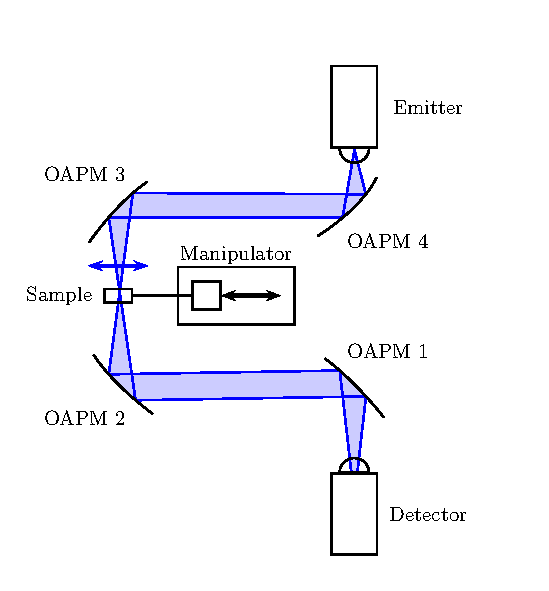
\includegraphics[width=0.5\linewidth]{images/3_chapter03/Setup-THz-TDS-HHI.pdf}}
    \qquad
    \subcaptionbox{\label{fig:2}}
        {\hspace*{-2em}\includestandalone[width=0.45\linewidth]{images/3_chapter03/sample_mount_simple}}
    
    \caption{a): The main components of the measurement setup which consists of four off-axis parabolic mirrors, the sample mounted on a translation stage(Manipulator) as well as the emitter and detector. b): The rotational sample mount where the blue arrow indicates the horizontal direction which is also the polarization plane of the incident radiation.}
    \label{fig:3_THz-TDS-HHI}
\end{figure}

Figure \ref{fig:HHI_pulse_example} (a) shows the time-domain signal from a reference measurement with 100 averages. Figure \ref{fig:HHI_pulse_example} (b) shows the spectrum of the pulse. We see that the spectrum contains frequency components up to around \SI{4.5}{\tera \hertz} with a signal peak at around \SI{500}{\giga \hertz}. Below \SI{200}{\giga \hertz} the signal becomes quite noisy.

\begin{figure}[H]
    \centering
    \includestandalone[scale=0.7]{images/3_chapter03/plots/pulse_example}
    \caption{Left: Example of a THz pulse from a reference measurement with 100 averages. Right: Spectrum of the pulse. The inset shows the first \si{\tera \hertz} of the spectrum.}
    \label{fig:HHI_pulse_example}
\end{figure}

\section{THz-TDS bowtie antenna setup}
\begin{figure}[H]
    \centering
    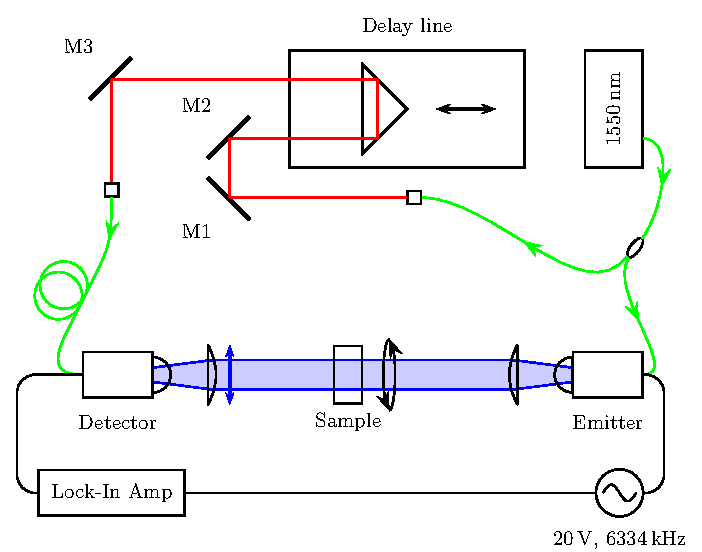
\includegraphics{images/3_chapter03/Setup-THz-TDS-Lab1.pdf}
    \caption{THz-TDS bowtie setup}
    \label{fig:THz_bowtie_setup}
\end{figure}

\section{Quasi-optical GHz setup}
For the characterization of the polymer waveplates a relatively low frequency setup was used. Specifically, the setup enables characterization of the sample in the millimeter and submillimeter wavelength range. A diagram of the setup is shown in figure \ref{fig:GHz_setup}. It mainly consists of a commercial vector network analyzer and different waveguide frequency extension units. The frequency extension units allow measurements to be performed in the following six frequency ranges: \SIrange[range-phrase=--]{50}{75}{\giga \hertz}, \SIrange[range-phrase=--]{75}{110}{\giga \hertz}, \SIrange[range-phrase=--]{110}{170}{\giga \hertz}, \SIrange[range-phrase=--]{140}{220}{\giga \hertz}, \SIrange[range-phrase=--]{220}{325}{\giga \hertz} and from \SIrange{325}{500}{\giga \hertz}. 

\begin{figure}[H]
    \centering
    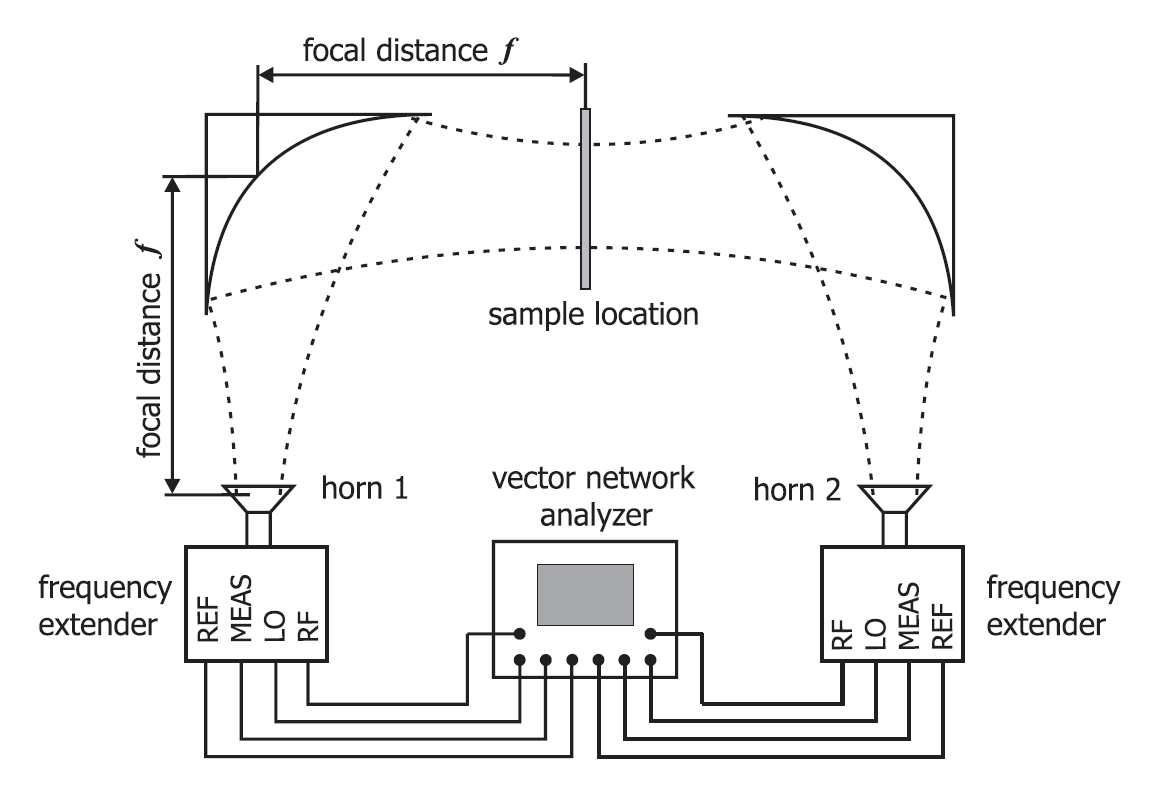
\includegraphics[scale=0.45]{images/3_chapter03/ghz.png}
    \caption{GHz setup}
    \label{fig:GHz_setup}
\end{figure}

